


Let's first consider $k_{||}v_{||}<< \nu<< \omega$

\begin{eqnarray}
     \frac{B}{A}=\frac{ \int ^{\infty} _{0}   dv \frac{v^4(\frac{v^2}{2v^2_{th}}-3/2) }{1-i\frac{\nu_0\cdot v_{th}^3}{\omega v^3}} e^{-m_sv^2/2T_s}
     }{\int ^{\infty} _{0}   dv \frac{v^4}{1-i\frac{\nu_0\cdot v_{th}^3}{\omega v^3}} e^{-m_sv^2/2T_s}
     }
\end{eqnarray}
There are $\omega$ on both sides, it is hard to solve for analytically. But one can get solution with ease when we take two extreme cases. 
\begin{enumerate}
    \item For $\frac{\nu_0}{\omega}\longrightarrow 0$
    \begin{eqnarray}
         \frac{B}{A}=\frac{ \int ^{\infty} _{0}   dv \cdot v^5(\frac{v^2}{2v^2_{th}}-3/2) (1+i\frac{\nu_0\cdot v_{th}^3}{\omega v^3}) e^{-m_sv^2/2T_s}
     }{\int ^{\infty} _{0}   dv\cdot v^5 (1+i\frac{\nu_0\cdot v_{th}^3}{\omega v^3}) e^{-m_sv^2/2T_s}
     }\\
     \frac{B}{A}=\frac{2 m v_{th}^2}{3 (T - m v_{th}^2)}
    \end{eqnarray}
    \item For $\frac{\nu_0}{\omega}\longrightarrow \infty$
    \begin{eqnarray}
         \frac{B}{A}=\frac{ \int ^{\infty} _{0}   dv \cdot v^7(\frac{v^2}{2v^2_{th}}-3/2) e^{-m_sv^2/2T_s}
     }{\int ^{\infty} _{0}   dv\cdot v^7 e^{-m_sv^2/2T_s}
     }\\
     \frac{B}{A}=\frac{4 m v_{th}^2}{3 (3 T - 2 m v_{th}^2)}
    \end{eqnarray}
\end{enumerate}

Now let's take $k_{||}v_{||}$ into consideration. The analysical solution is almost impossible. We will do it purely numerically, Recall Equation \ref{eq:omega}. We have: 

\begin{eqnarray}
     \frac{B}{A}=\frac{\int^{\pi}_{0}d\theta \int ^{\infty} _{0}   dv \frac{v^4(\frac{v^2}{2v^2_{th}}-3/2) sin\theta cos^2\theta}{1-\frac{k_{||}v cos(\theta)}{\omega}-i\frac{\nu_0\cdot v_{th}^3}{\omega v^3}} e^{-m_sv^2/2T_s}
     }{\int^{\pi}_{0}d\theta \int ^{\infty} _{0}   dv \frac{v^4 sin\theta cos^2\theta}{1-\frac{k_{||}v cos(\theta)}{\omega}-i\frac{\nu_0\cdot v_{th}^3}{\omega v^3}} e^{-m_sv^2/2T_s}
     }
\end{eqnarray}
Solve for $\omega$ and substitute $s=\frac{v}{v_{th}}$,one can get
\begin{eqnarray}
     \omega=\omega_{*n}+\frac{B}{A}\omega_{*T}\\
     \frac{B}{A}=\frac{\int^{\pi}_{0}d\theta \int ^{\infty} _{0}   dv \frac{s^4(\frac{s^2}{2}-3/2) sin\theta cos^2\theta}{1-\frac{k_{||}s\cdot v_{th} cos(\theta)}{\omega}-i\frac{\nu_0 }{\omega s^3}} e^{-s^2/2}
     }{\int^{\pi}_{0}d\theta \int ^{\infty} _{0}   dv \frac{s^4 sin\theta cos^2\theta}{1-\frac{k_{||}s\cdot v_{th} cos(\theta)}{\omega}-i\frac{\nu_0 }{\omega s^3}} e^{-s^2/2}
     }
     \label{eq:B/A}
\end{eqnarray}

And the $\frac{B}{A}$ only depends on the two following to quantities: $\frac{k_{||}v_{th}}{\omega}$, $\frac{\nu_0}{\omega}$.

Using the following number for calculation
\begin{eqnarray}
     \eta=\frac{\omega_{*T}}{\omega_{*n}}=1.5\\
     q=4\\
     T_e=0.4keV\ \ \ (in GENE)\\
     k_{||}=\frac{in}{R}(1-\frac{m}{nq})
     v_{th}=\\
     L_s=8m\\
     k_y=0.1\\
     kx=0\\
     k_{||}=k_y(GENE)/L_s=1/80 m^{-1}
\end{eqnarray}

\begin{eqnarray}
     \omega=\omega_{*n}(1+1.5\frac{B}{A})
\end{eqnarray}

One can calculate the it numerically using Mathematica. 

Here is the $k_{||}=0$ shown in Figure \ref{fig:k_0}

\begin{figure}[h] \centering
        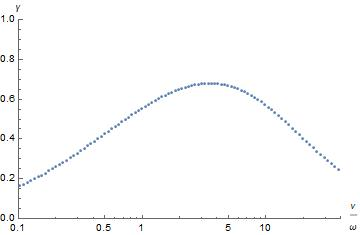
\includegraphics[width=1\textwidth]{Image/kpara=0.jpg}
        \caption{The growth rate of MTM with $k_{||}$=0}
        \label{fig:k_0}
\end{figure}


The Plot of growth rate with different k is shown in Figure \ref{fig:k_diff}

\begin{figure}[h] \centering
        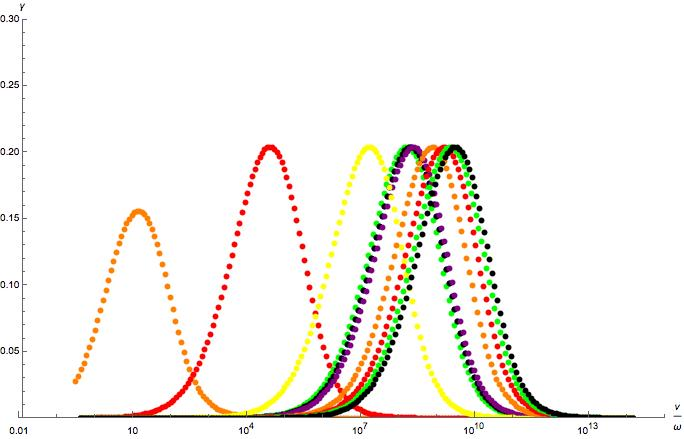
\includegraphics[width=1\textwidth]{Image/k_diff.jpeg}
        \caption{The growth rate of MTM with different k}
        \label{fig:k_diff}
\end{figure}

As Figure \ref{fig:k_peak} shown, the peak of the growth rate is sensitive of change of k near 0.

\begin{figure}[h] \centering
        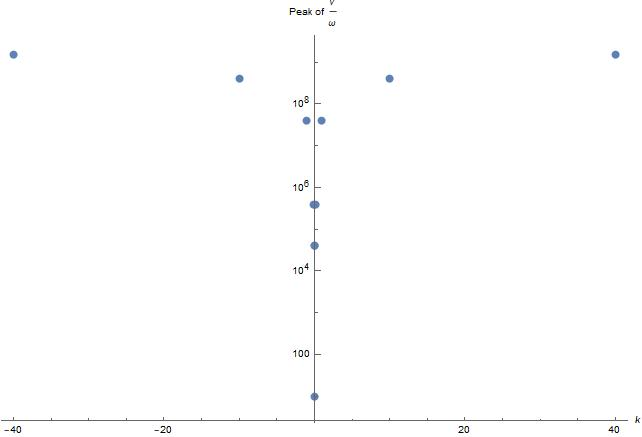
\includegraphics[width=1\textwidth]{Image/k_peak.jpg}
        \caption{The growth rate peak of MTM with changing k}
        \label{fig:k_peak}
\end{figure}
